% ===========================================================================
% OWNER: M3 (Zarpash Nasim)
% GRADED BY: Form 3 #4 Requirements & acceptance criteria (15)
% DRAW FROM: docs/02-Requirements/functional.md, non-functional.md, scope-boundary.md, docs/03-Design/certificate-contract.md, eval/schema/report.schema.json, fixtures/od-fixture/ground_truth.json
% NOTE: Every FR/NFR needs an objective acceptance check; the traceability table links FR -> module -> file -> test
% Rules: mid-eval-report/CLAUDE.md. Do not edit a file you do not own.
% ===========================================================================
\chapter{Software Requirements}
\section{User Interactions / Use Cases}
FlakeTrace has two actors. A \textbf{Developer} invokes it directly against a failing test
they are investigating. A \textbf{CI Pipeline} invokes it the same way, on demand for a known
failing test rather than on every build --- Non-Functional Requirement NFR-1 (Section
\ref{ch4:sec:nfr}) is the reason: our stakeholders' own CI-time budgets rule out running it on
every successful build. Both actors drive the same seven use cases (Figure
\ref{ch4:fig:usecases}): submit a diagnosis request, through to receiving a typed certificate.

\section{Use Case Diagram}
% Use case diagram (M3): diagrams/m3/use_cases.puml -> figures/m3/use_cases.png
\begin{figure}[H]\centering
  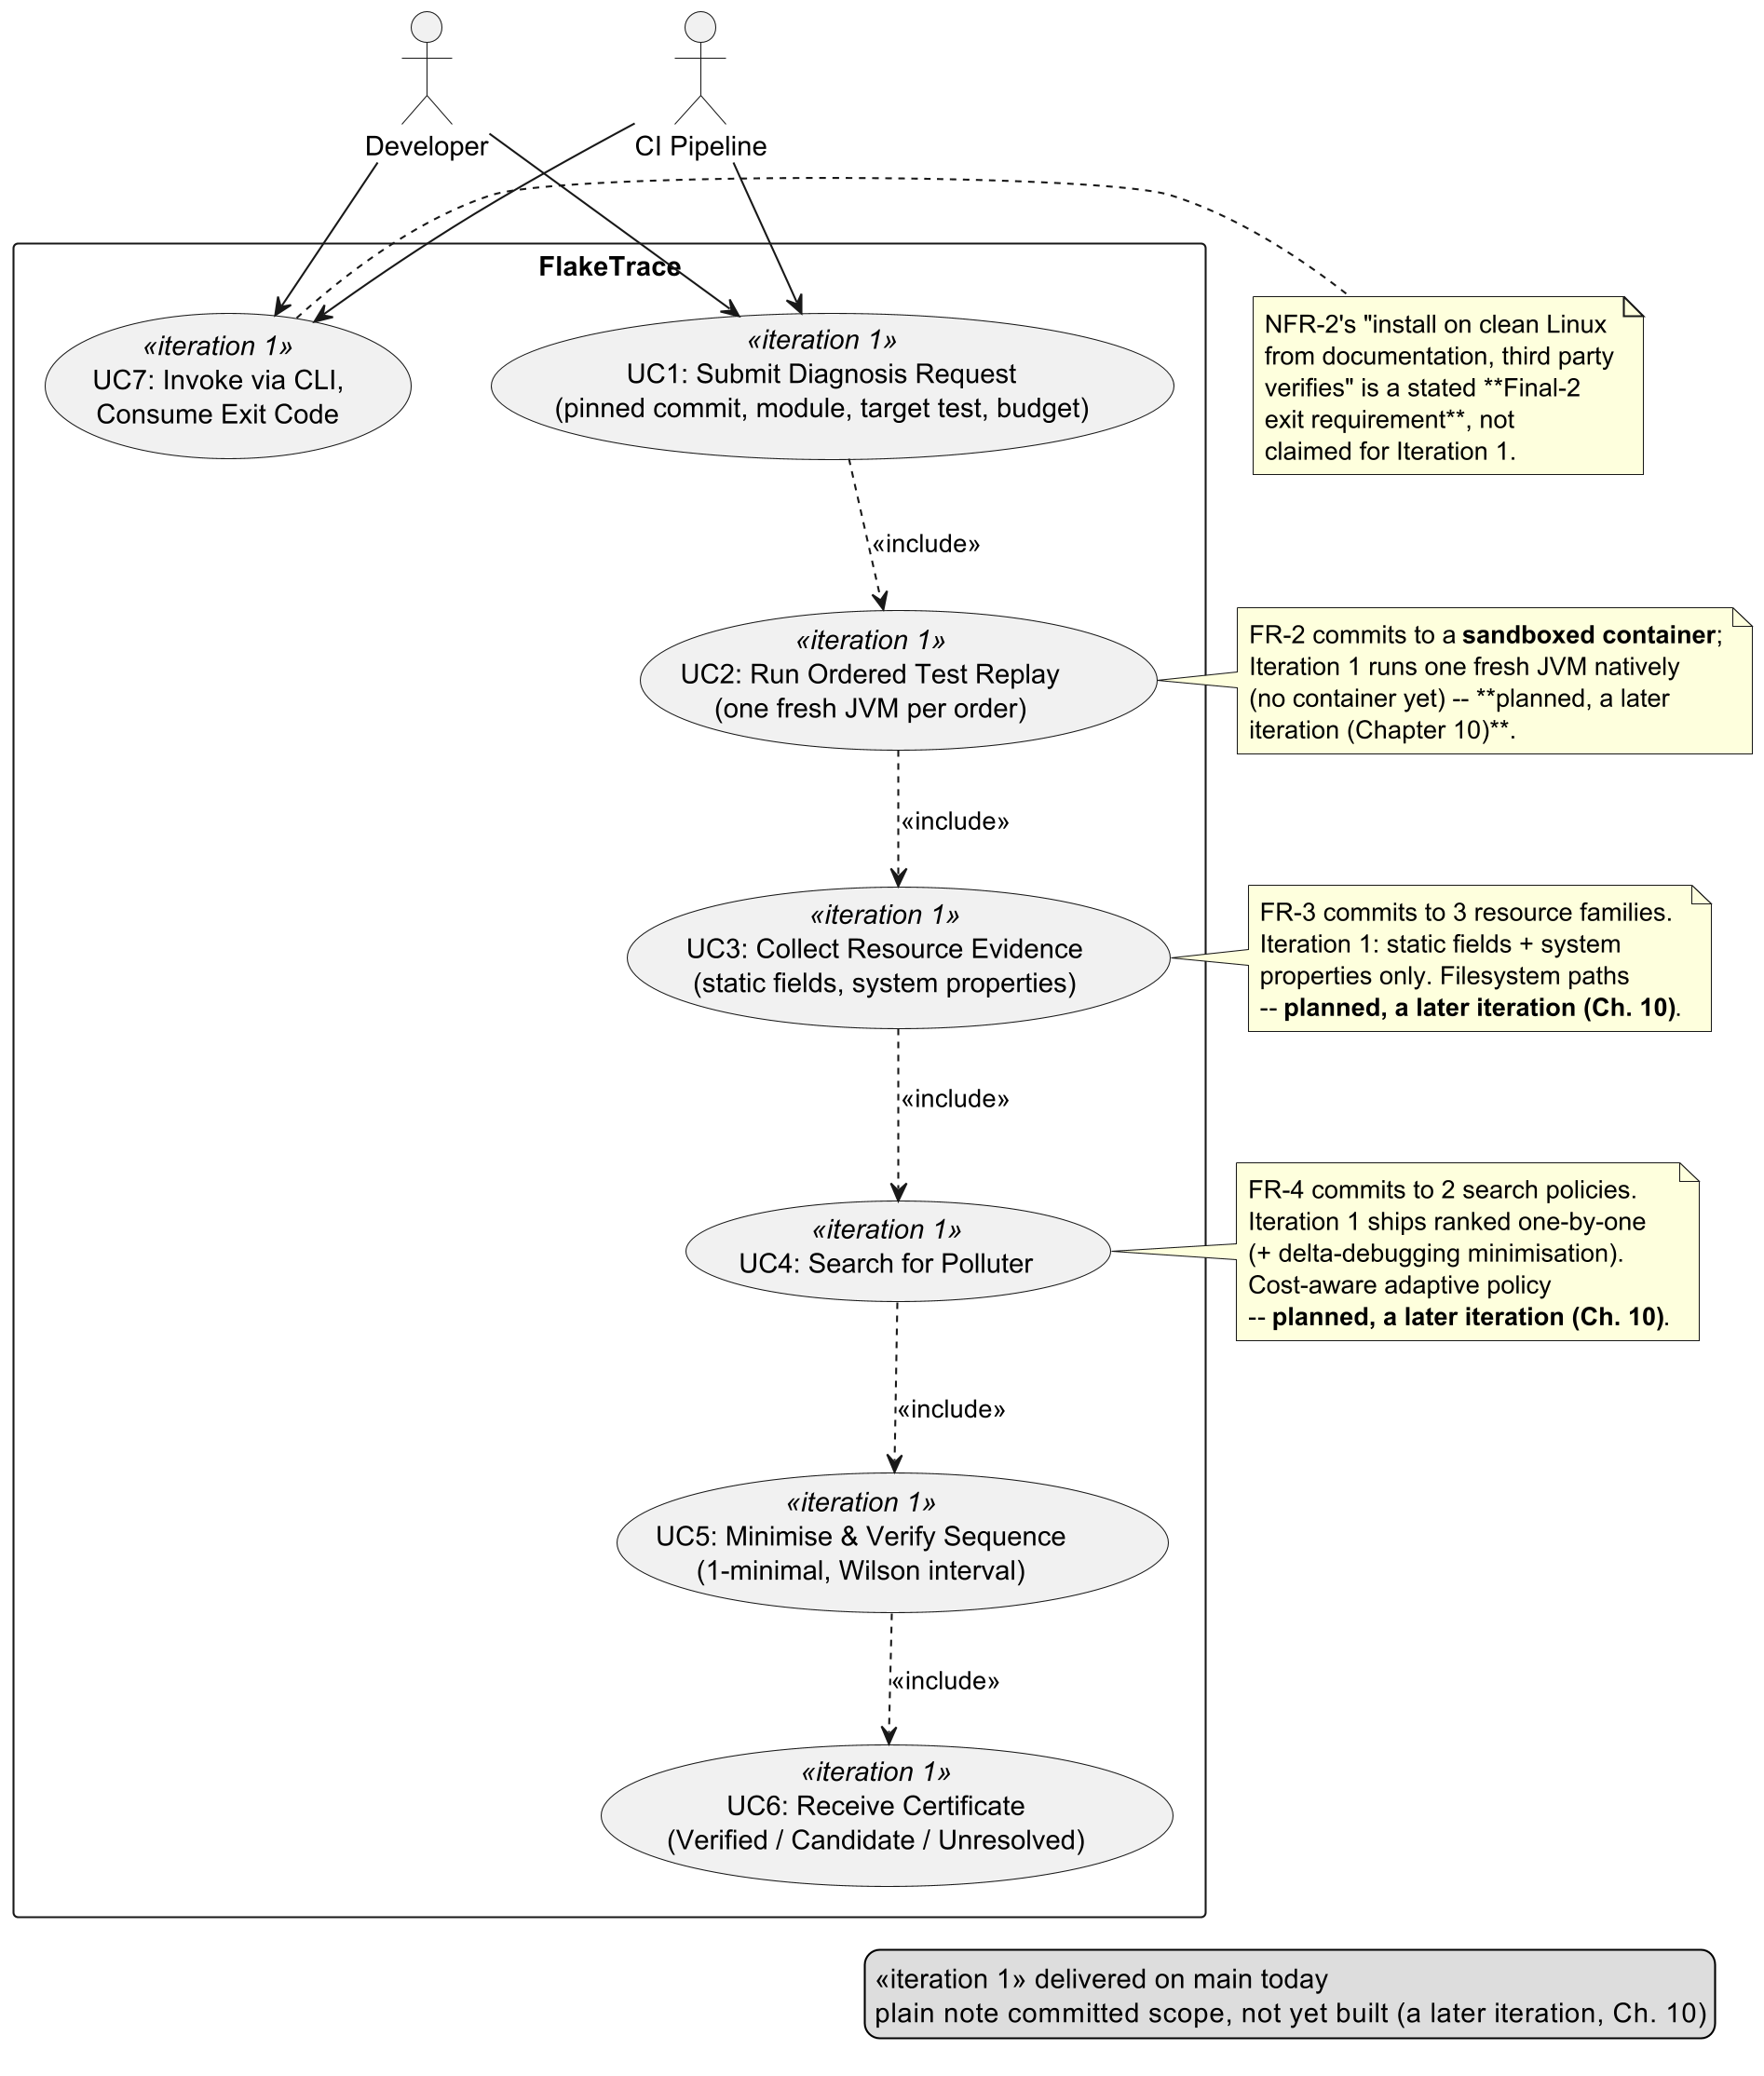
\includegraphics[width=0.85\textwidth]{figures/m3/use_cases}
  \caption{FlakeTrace use case diagram}\label{ch4:fig:usecases}
\end{figure}
Figure \ref{ch4:fig:usecases} shows the whole committed project, not only what Iteration 1
delivers: every use case carries the \texttt{<<iteration 1>>} stereotype because all seven are
implemented on \texttt{main} today, but the attached notes mark exactly which part of each
FR's full commitment is still FYP-2 work (container sandboxing, the filesystem resource
family, the cost-aware adaptive search policy, and NFR-2's clean-machine deployment check) ---
checked against the real code (\texttt{runner/}, \texttt{evidence/}) while drawing this
diagram, not assumed from the proposal.
\section{Detailed Use Cases}
\section{Functional Requirements}
\subsection{Module 1}
\subsection{Module 2}
\section{Non-Functional Requirements}\label{ch4:sec:nfr}
\subsection{Reliability}
\subsection{Usability}
\subsection{Performance}
\subsection{Security}
\section{Acceptance Criteria}
Define objective acceptance checks for important requirements.
\section{Requirements Traceability}
Trace important requirements to modules, design elements, implementation, and tests.
